% CVPR 2027 review-mode manuscript.
\documentclass[10pt,twocolumn,letterpaper]{article}
\usepackage[review]{cvpr}
%% This file contains a number of tweaks that are typically applied to the main document.
%% They are not enabled by default, but can be enabled by uncommenting the relevant lines.

%%
%% Inline annotations; for predefined colors, refer to "dvipsnames" in the xcolor package:
%% https://tinyurl.com/overleaf-colors
%%
\newcommand{\red}[1]{{\color{red}#1}}
\newcommand{\todo}[1]{{\color{red}#1}}
\newcommand{\TODO}[1]{\textbf{\color{red}[TODO: #1]}}
%%
%% disable for camera ready / submission by uncommenting these lines  
%%
% \renewcommand{\TODO}[1]{}
% \renewcommand{\todo}[1]{#1}

%%
%% work harder in optimizing text layout. Typically shrinks text by 1/6 of page, enable
%% it at the very end of the writing process, when you are just above the page limit
%%
% \usepackage{microtype}

%%
%% fine-tune paragraph spacing
%%
% \renewcommand{\paragraph}[1]{\vspace{.5em}\noindent\textbf{#1.}}

%%
%% globally adjusts space between figure and caption
%%
% \setlength{\abovecaptionskip}{.5em}


%%
%% Allows "the use of \paper to refer to the project name"
%% with automatic management of space at the end of the word
%%
% \usepackage{xspace}
% \newcommand{\paper}{ProjectName\xspace}

%%
%% Commonly used math definitions
%%
% \DeclareMathOperator*{\argmin}{arg\,min}
% \DeclareMathOperator*{\argmax}{arg\,max}

%%
%% Tigthen underline
%%
% \usepackage{soul}
% \setuldepth{foobar}
% R90: reclaim the final Conclusion line onto p8 after adding Figure 1.
\linespread{0.845}

\usepackage{booktabs}
\usepackage{amsmath,amssymb}
\usepackage{graphicx}
\definecolor{cvprblue}{rgb}{0.21,0.49,0.74}
\usepackage[pagebackref,breaklinks,colorlinks,allcolors=cvprblue]{hyperref}
\newcounter{auditbox}

\def\paperID{*****}
\def\confName{CVPR}
\def\confYear{2027}

\title{When Does the Wiring Help? Path Survival and Density\\ Gating Govern Topology Advantage in Connectome Vision}

\author{Anonymous}

\setlength{\floatsep}{4pt plus 1pt minus 2pt}
\setlength{\textfloatsep}{6pt plus 1pt minus 2pt}
\setlength{\intextsep}{4pt plus 1pt minus 2pt}
\begin{document}
\maketitle

\begin{abstract}
Does connectome wiring topology confer a measurable advantage to visual
computation -- and if so, \emph{when}? Published answers now disagree across
systems: fixed-connectome models report gains at matched wiring cost in the
adult fly visual system~\cite{structurealone2026}, a degree-preserving control
erases those gains under shared initialisation~\cite{toposens2026}, the larval
connectome shows no advantage over its own degree-preserving
shuffle~\cite{larvanull2026}, and a whole-connectome network reports gains
again on cognitive tasks~\cite{cho2026whole}. We treat this disagreement as
the object of study and ask which structural mechanism gates the advantage.
We preregister an adjudication on three scales: a controlled 96-node graph
whose XOR label is solvable only through an injected two-hop convergence
motif, evaluated under a nested ladder of null generators with machine-checked
invariants; a single-variable density sweep on a real MaleCNS visual
subgraph; and a density$\times$path-survival grid that manipulates the two
candidate mechanisms orthogonally. The answer is a \emph{two-factor gate}. On
the controlled graph the real graph reaches $0.8152$ held-out accuracy while
every null rung sits at chance ($0.4795$--$0.5133$, $q=0.0002$), yet rungs
differ by at most $0.0244$: what matters is whether the control preserves the
task-relevant path. A task-aware null protecting the 18 motif edges matches
the real graph ($0.8346$ vs.\ $0.8371$, $q=0.40$), a motif-dose ladder
collapses once 9 or fewer edges survive, and survival is necessary but not
sufficient without input--path alignment. On real wiring the second factor appears:
in-degree alone decides whether the task is solvable at all (chance at mean
in-degree $58.4$; $0.9863$ at $4.0$), and the grid confirms the interaction --
a dense background erases even a fully protected path, while a sparse
background cannot rescue a destroyed one. A real image-classification test
shows the wiring prior is not a competitive bias, bounding the claim's scope.
We release a generator standard with per-rung invariant assertions and a
survival-count audit: control construction, not topology order, explains the
conflicting reports.
\end{abstract}

% R97 P0-1/P0-4: survival-count and global-match columns added to the main
% matrix. Survival counts are a POST-HOC deterministic replay of the frozen
% null generators (no new training, no new seeds, no label access).
% Oracle row is POST-HOC EXPLORATORY (10 frozen seeds, same protocol).
% Neither addition enters the preregistered BH/CI significance family.
%
% Tables derived from the recorded measurements.

\begin{table}[t]\centering\caption{Main matrix, ten frozen seeds. All real-minus-condition
differences have 95\% bootstrap CIs excluding zero and BH $q=0.0002$; chance $=0.5$.
$|P\cap A|$ is the mean number of the 18 objectively defined two-hop motif edges
surviving in each null (16, 16, 16, 8, 16 instances for L0--L4); $\Delta_{\rm conv2}$ is
$|\overline{\mathrm{conv2}}(A_{\rm null})-\mathrm{conv2}(A_{\rm real})|$, with
$\mathrm{conv2}_{\rm real}=178$ and the mean taken over instances.
The two new columns are \emph{post-hoc re-analysis} of graphs already used for
the accuracy measurements, not a new experiment. Oracle is a \emph{post-hoc
exploratory} 10-seed probe on the identical dataset and protocol; neither addition
enters the preregistered significance family.}\label{tab:main}\small
\resizebox{\linewidth}{!}{\begin{tabular}{lccccc}\toprule
Condition & Mean acc. & Seed var. & $\Delta$ (95\% CI) & $|P\cap A|$ & $\Delta_{\rm conv2}$ \\ \midrule
Real graph & 0.8152 & 2.10e-04 & -- & 18.00 & 0 \\
$A=0$ & 0.4879 & 6.61e-04 & $0.3273$ [0.3043,0.3463] & 0.00 & 178.00 \\
L0 ER & 0.4795 & 3.50e-04 & $0.3357$ [0.3191,0.3525] & 0.44 & 24.88 \\
L1 +degree & 0.5039 & 3.55e-04 & $0.3113$ [0.2947,0.3275] & 1.13 & 0.13 \\
L2 +module & 0.4961 & 3.13e-04 & $0.3191$ [0.3021,0.3352] & 13.50 & 5.94 \\
L3 +triad & 0.4986 & 7.48e-05 & $0.3166$ [0.3027,0.3293] & 13.38 & 0.50 \\
L4 indep. (control) & 0.5016 & 2.63e-04 & $0.3137$ [0.2984,0.3293] & 0.69 & 6.00 \\
Motif only (upper bnd) & 0.8348 & 2.35e-04 & $-0.0195$ [-0.0307,-0.0086] & 6.00 & -- \\
Shuffled node$\to$input & 0.5133 & 1.54e-04 & $0.3020$ [0.2865,0.3162] & 18.00 & 0 \\
\midrule
\multicolumn{6}{l}{\emph{Post-hoc exploratory, not in the preregistered family:}}\\
Oracle (both sources given) & 0.7859 & 6.12e-05 & -- & -- & -- \\
\bottomrule\end{tabular}}\end{table}

\begin{table}[t]\centering\caption{Null-ladder invariants (maximum violation over instances).
L4 violates every invariant and is therefore a matched control, not a rung.}\label{tab:invariants}\small
\begin{tabular}{lrrrr}\toprule Rung & Edges & Degree & Blocks & Triad L1 \\ \midrule
L0 & 0 & 95 & 53 & 484 \\
L1 & 0 & 0 & 47 & 756 \\
L2 & 0 & 0 & 0 & 1826 \\
L3 & 0 & 0 & 0 & 20 \\
L4 & 28 & 93 & 39 & 4836 \\
\bottomrule\end{tabular}\end{table}

\begin{table}[t]\centering\caption{Robustness: $\Delta$ = acc(real) $-$ acc(L1)
under two input-noise levels and two message-passing depths.}\label{tab:robust}\small
\begin{tabular}{lcc}\toprule Noise / depth & 2 rounds & 3 rounds \\ \midrule
0.05 & 0.3652 & 0.3561 \\
0.2 & 0.1406 & 0.2064 \\
\bottomrule\end{tabular}\end{table}

% Tables derived from the recorded measurements.

\begin{table}[t]\centering\caption{Task-aware null and motif-dose controls, 10 frozen seeds. 
$\Delta$ is acc(real) minus acc(condition); CIs are paired seed-level bootstrap; $q$ is BH-adjusted. 
The task-aware null keeps all 18 motif edges and randomises only the background.}\label{tab:taskaware}\small
\resizebox{\linewidth}{!}{\begin{tabular}{lccc}\toprule Condition & Mean acc. & $\Delta$ (95\% CI) & $q$ \\ \midrule
Real graph & 0.8371 & -- & -- \\
$A=0$ & 0.5020 & $0.3352$ [0.3172,0.3521] & 0.00032 \\
Task-aware null (18/18 kept) & 0.8346 & $0.0025$ [-0.0025,0.0084] & 0.40132 \\
Background-only null (14/18 kept) & 0.8260 & $0.0111$ [-0.0035,0.0268] & 0.18122 \\
Strong null (0/18 kept) & 0.4920 & $0.3451$ [0.3316,0.3590] & 0.00032 \\
Motif removed (0/18) & 0.5117 & $0.3254$ [0.3123,0.3395] & 0.00032 \\
Motif kept 14/18 & 0.8316 & $0.0055$ [-0.0020,0.0135] & 0.18122 \\
Motif kept 9/18 & 0.4988 & $0.3383$ [0.3246,0.3504] & 0.00032 \\
Motif kept 4/18 & 0.5104 & $0.3268$ [0.3168,0.3377] & 0.00032 \\
\bottomrule\end{tabular}}\end{table}

% Tables derived from the recorded measurements.

\begin{table}[t]\centering
\caption{Real MaleCNS v1.0 visual subgraph, six frozen seeds. Dense: 768 nodes / 48,723 edges / mean in-degree 63.4. Sparse: the same graph with the four highest-weight in-edges per node retained, 3,072 edges / mean in-degree 4.0.}\label{tab:real}\small
\begin{tabular}{lcc}\toprule Condition & Dense & Sparse \\ \midrule
Real graph & 0.5186 & 0.6423 \\
$A=0$ & 0.5264 & 0.5283 \\
Degree-preserving & 0.5088 & 0.6162 \\
Task-aware & 0.5156 & 0.5850 \\
Motif removed & 0.5306 & 0.5160 \\
\bottomrule\end{tabular}
\end{table}

\begin{table}[t]\centering
\caption{Powered held-out study (20 graphs). Features are significant after Benjamini--Hochberg correction over the 12-feature family. LOGO = leave-one-graph-out.}\label{tab:heldout}\small
\begin{tabular}{lc}\toprule Quantity & Value \\ \midrule
Graphs (intact / motif-degraded) & 20 (10 / 10) \\
Delta sign counts (positive / non-positive) & 12 / 8 \\
Features significant after BH ($q<0.05$) & 8 of 12 \\
LOGO magnitude MAE & 0.1046 \\
Constant-mean baseline MAE & 0.1635 \\
LOGO sign agreement & 0.60 \\
Majority-class sign baseline & 0.60 \\
\bottomrule\end{tabular}
\end{table}

% Tables derived from the recorded measurements.

\begin{table}[t]\centering
\caption{Single-variable density sweep on a real MaleCNS v1.0 visual subgraph, six frozen seeds. Only the number of retained in-edges per node ($k$) changes; readout, epochs, width, learning rate, seeds and motif are fixed. Oracle: $1.0000$ on all seeds.}\label{tab:density}\small
\resizebox{\linewidth}{!}{\begin{tabular}{lcc|cccc}\toprule
$k$ & edges & in-deg & real & $A\!=\!0$ & deg-null & task-aware \\ \midrule
dense & 44,815 & 58.4 & 0.5049 & 0.5062 & 0.4977 & 0.4984 \\
63 & 37,634 & 49.0 & 0.4886 & 0.5062 & 0.5111 & 0.5029 \\
16 & 12,186 & 15.9 & 0.5075 & 0.5062 & 0.5059 & 0.4958 \\
8 & 6,144 & 8.0 & 0.6227 & 0.5062 & 0.4932 & 0.5407 \\
4 & 3,072 & 4.0 & 0.9863 & 0.5062 & 0.5133 & 0.9027 \\
2 & 1,536 & 2.0 & 0.9987 & 0.5062 & 0.5029 & 0.9971 \\
\bottomrule\end{tabular}}
\end{table}

\begin{table}[t]\centering
\caption{Real image classification (\texttt{sklearn} digits, 10 classes, 1078/359/360 split) with a 768-node MaleCNS visual subgraph as a fixed prior, six seeds. $\Delta$ is real minus condition with a 95\% paired bootstrap interval.}\label{tab:visual}\small
\resizebox{\linewidth}{!}{\begin{tabular}{lccc}\toprule
Condition & mean acc. & 95\% CI & $\Delta$ (95\% CI) \\ \midrule
Real graph & 0.7185 & [0.6856,0.7542] & -- \\
Degree-preserving null & 0.7190 & [0.6884,0.7495] & $-0.0005$ [-0.0412,+0.0440] \\
$A=0$ (no graph) & 0.6190 & [0.5708,0.6648] & $+0.0995$ [+0.0556,+0.1648] \\
Task-aware null & 0.7333 & [0.7088,0.7593] & $-0.0148$ [-0.0278,-0.0009] \\
Non-graph MLP & 0.9722 & [0.9699,0.9741] & $-0.2537$ [-0.2861,-0.2176] \\
\bottomrule\end{tabular}}
\end{table}

\begin{table}[t]
  \centering
  \caption{Density$\times$path-survival grid on the
  controlled graph family (pre-registered; six paired seeds). Effect = seed-paired
  held-out accuracy minus the no-graph control; 95\% bootstrap intervals are shown as
  error bars in Fig.~\ref{fig:grid}. The advantage requires both factors: full survival
  at base density replicates the main effect, the highest density erases even $k{=}18$,
  and $k{=}9$ already collapses at base density.}
  \label{tab:grid}
  \small
  \begin{tabular}{lccc}
    \toprule
    Mean in-degree & $k{=}18$ & $k{=}9$ & $k{=}0$ \\
    \midrule
    $s=1$ ($1.5$) & $+0.2396$ & $-0.0479$ & $-0.0186$ \\
    $s=8$ ($9.5$) & $-0.0052$ & $-0.0156$ & $-0.0251$ \\
    $s=32$ ($24.3$) & $-0.0094$ & $-0.0042$ & $-0.0215$ \\
    $s=64$ ($34.8$) & $-0.0247$ & $-0.0326$ & $-0.0290$ \\
    \bottomrule
  \end{tabular}
\end{table}

% R97: two-coordinate taxonomy (P0-3), literature comparison (P0-5),
% and the survival-count audit algorithm (writing surgery item 3).

\begin{table}[t]\centering\caption{Two orthogonal coordinates of control design.
Columns increase the number of matched \emph{global} invariants (rung order);
rows vary whether the \emph{task-relevant path} $P$ is preserved. $L^*$
is not on the rung ladder: path preservation is a different axis from
statistical order. Accuracies are from the main matrix (Table~\ref{tab:main})
and the task-aware companion run (Table~\ref{tab:taskaware}); they are not a
single pooled family.}\label{tab:taxonomy}\footnotesize
\resizebox{\linewidth}{!}{\begin{tabular}{lccccc}\toprule
 & L0 & L1 & L2 & L3 & $L^*$ (path kept) \\ \midrule
Global invariants matched & 0 & 1 & 2 & 3 & varies \\
$|P\cap A|$ (mean) & 0.44 & 1.13 & 13.50 & 13.38 & 18 \\
$\Delta_{\rm conv2}$ & 24.88 & 0.13 & 5.94 & 0.50 & -- \\
Acc.\ (chance $=0.5$) & 0.4795 & 0.5039 & 0.4961 & 0.4986 & 0.8346 \\
\bottomrule\end{tabular}}\end{table}

\begin{table}[t]\centering\caption{Literature comparison. All entries describing
other studies are \emph{we estimate / proxy} statements, not claims about
their internal results; where a quantity is not reported in the accessible
record we say so rather than infer it. Task-sensitivity gate and path-survival
proxies are our own protocol's terms applied as an external reading aid.}
\label{tab:literature}\footnotesize
\resizebox{\linewidth}{!}{\begin{tabular}{llll}\toprule
Work & Reported claim & Null family (as described) & Path-survival proxy$^\dagger$ \\ \midrule
\cite{structurealone2026} & gains at matched wiring cost & wiring-cost-matched ensembles & we estimate: not reported \\
\cite{toposens2026} & advantage vanishes early & degree-preserving, shared init & we estimate: low (degree swap) \\
\cite{flygm2026} & motor-domain positive & not comparable to ours & we estimate: not reported \\
\cite{flyhack2026} & ensemble-level lesion audit & lesion, not null rewiring & we estimate: not applicable \\
This work & control protocol is the confound & nested L0--L3 $+$ $L^*$ & measured: 0.44--18 of 18 \\
\bottomrule\end{tabular}}
\\[2pt]\raggedright\scriptsize
$^\dagger$Our proxy, computed by applying our survival-count definition to the
control construction as described, not a measured quantity of those studies.
No entry asserts that a prior conclusion is wrong; different null families
answer different questions.
\end{table}


\section{Introduction}
\label{sec:intro}

Connectome-constrained models hold a distinctive promise for vision: if the
wiring diagram of a biological visual system is known, a model can inherit it
as an inductive bias instead of learning it. That promise now comes with a
puzzle -- the published evidence disagrees \emph{across systems, not just
within them}. Fixed-connectome models with learned scalar gains report
efficient visual computation at matched wiring cost~\cite{structurealone2026};
a strict degree-preserving null with shared initialisation removes much of
that advantage in the same system~\cite{toposens2026}; the complete larval
connectome, used as a fixed reservoir, shows no advantage over its own
degree-preserving shuffle once the seed count is raised from five to
fifteen~\cite{larvanull2026}; an adult whole-connectome network reports large
gains over degree-preserving rewires on cognitive tasks~\cite{cho2026whole};
and an embodied study shows that which edges a null preserves at the
sensory--motor boundary can flip the sign of an evolutionary
comparison~\cite{park2026nullboundary}. Motor-domain positives and
ensemble-level lesion audits further complicate the
picture~\cite{flygm2026,flyhack2026}.

We argue these studies are not contradictory once the question is asked at
the right level. They differ in the null family, the training horizon, the
task, and -- critically -- the \emph{regime} of the graph being compared:
adult visual studies operate on sparse, cell-type-resolved circuits, while
reservoir-style studies project dense connectome subgraphs onto their inputs.
The field lacks a controlled comparison in which the null model itself is the
experimental variable. We treat the control generator as a
\emph{measurable object}: rather than proposing a new visual backbone, we
vary the generator under controlled causal interventions, validate each
instance against machine-checked invariants, and ask which structural
mechanism -- path survival, wiring density, or their interaction -- gates the
advantage. The object of study is the comparison protocol itself.

We preregister such a comparison on three scales. First, a \emph{nested
ladder} of null graphs on a controlled 96-node circuit: the rungs match the
edge count (L0), per-node in/out degree (L1), module-pair edge counts (L2),
and the full directed triad census (L3), with an independent graph from the
same generator (L4) as a matched control; every rung carries explicit
invariant assertions. The paired task is an XOR of two distant source nodes,
solvable only through an injected two-hop convergence motif, so removing the
graph (or the relevant edges) provably removes the only information path.
Ten frozen seeds, paired bootstrap intervals, Benjamini--Hochberg
correction~\cite{benjamini1995} and a leave-one-graph-out evaluation of
training-free statistics complete the protocol. Second, a
\emph{single-variable density sweep} on a real MaleCNS visual subgraph, which
holds every factor fixed except the number of retained in-edges per node.
Third, a pre-registered \emph{density$\times$path-survival grid} on the
controlled family that manipulates the two candidate mechanisms orthogonally.
Three outcomes were admissible \emph{a priori}: (i) a monotone ladder that
localises the advantage; (ii) a preregistered null result; or (iii) a
diagnostic outcome in which the ladder itself proves inadequate.

We observe outcome (iii), and it is diagnostic. The effect is large and
unambiguous, but every rung erases it to nearly the same degree -- because
the rungs control a quantity orthogonal to the one that matters. Tracing that
orthogonality, and crossing it with the real-wiring sweep, yields the
gating mechanism. Our contributions are:

\begin{itemize}
\item \textbf{The survival--match gap (controlled mechanism).} A large,
  reproducible effect ($0.8152$ vs.\ $0.4795$--$0.5133$, $q=0.0002$) that no
  order of global-statistic matching can localise: rungs differ by at most
  $0.0244$, an order of magnitude below the effect, and monotonicity is
  violated. The two-coordinate taxonomy (Table~\ref{tab:taxonomy}) separates
  matched statistical \emph{order} from task-relevant \emph{path survival};
  a task-aware null $L^*$ restores the advantage, and survival is necessary
  but not sufficient (\S\ref{sec:survival}).
\item \textbf{The density gate (real-wiring mechanism).} A single-variable
  sweep on real MaleCNS wiring shows in-degree alone determines whether the
  diagnostic task is solvable at all -- chance at mean in-degree $58.4$,
  near-ceiling at $4.0$ -- with an oracle control ruling out a label
  explanation, and the task-aware null echoing the controlled result at low
  density (\S\ref{sec:density}).
\item \textbf{The two-factor interaction.} A pre-registered
  density$\times$survival grid on the controlled family confirms that the two
  factors gate jointly: a dense background erases even a fully protected
  path, and a sparse background cannot rescue a destroyed one
  (Table~\ref{tab:grid}; \S\ref{sec:grid}). The grid unifies the positive
  controlled result, the real-wiring sweep, and the published cross-system
  disagreement into one mechanism.
\item \textbf{A reusable standard.} Four nested rungs plus a matched control
  with machine-checked invariants, an explicit survival-count audit
  (Algorithm~\ref{alg:audit}), a repair recipe (\S\ref{sec:repair}), and a
  shared-initialisation, multi-seed, corrected statistical protocol. A powered
  20-graph study keeps 8 of 12 features significant after correction, with
  magnitude prediction beating a constant baseline by 36\% but sign prediction
  equal to the majority-class baseline.
\end{itemize}

\section{Related Work}
\label{sec:related}

\paragraph{Connectome-constrained vision.}
The fly visual system has become a testbed for wiring-constrained models.
Lappalainen et al.~\cite{lappalainen2024} introduced a connectome-constrained
deep mechanistic network with cell-type-resolved connectivity and an
optic-flow task, together with pretrained models and reproduction notebooks.
Subsequent work fixed the graph and learned only synaptic gains or a linear
readout~\cite{structurealone2026}, and whole-brain
directed message-passing controllers have been studied in the motor
domain~\cite{flygm2026}. The MaleCNS v1.0 release provides a publicly
licensed full adult male CNS connectome~\cite{malecns2026}, and the FlyWire
female brain connectome offers a separate, non-interchangeable resource
with different neuron and synapse counts~\cite{dorkenwald2024}.

\paragraph{Null models and network motifs.}
Degree-preserving randomisation and edge swaps are standard tools for
separating topology from lower-order
constraints~\cite{maslov2002,milo2002}; the sixteen-class directed triad
census provides a classical higher-order description~\cite{wasserman1994,
hagberg2008}. The closest prior work~\cite{toposens2026} applies a
degree-preserving null with shared initialisation to a connectome-constrained
network and reports that early-training topological advantages largely
disappear; its stated limitations name longer training horizons, a broader
task set and higher-order nulls as future work -- precisely the axes our
ladder varies. Ensemble-level interventions~\cite{flyhack2026} and
reconstruction-variation audits~\cite{reconvar2026} address orthogonal
questions and do not test a nested null ladder.

\paragraph{Evaluation protocol.}
Our task construction follows synthetic structure-sensitivity tests in graph
learning, where a label is solvable only through a specified relational
path~\cite{kipf2017,xu2019}. We additionally require a leakage probe (a linear
classifier on raw or pooled features stays at chance) and a graph-removal
ablation that collapses the model -- distinguishing \emph{structural}
advantage from mere capacity.

\section{Method}
\label{sec:method}

\subsection{Controlled graph and data provenance}
\label{sec:graph}

We use a 96-node directed graph with eight modules, intra-module edge
probability $p_{\text{in}}=0.06$, inter-module probability
$p_{\text{out}}=0.004$, and four injected two-hop convergence motifs
$(\text{sources } a,b)\to \text{relay } r\to \text{sinks } S$ with all
$a\!\to\!S$ and $b\!\to\!S$ edges removed. The resulting graph has 123 edges.
Module sizes $[25,17,12,11,11,7,7,6]$ follow the eight most frequent
cell classes in the public MaleCNS v1.0 annotation table (minimum confidence
0.5; 14.5\,MB, CC-BY~4.0~\cite{malecns2026}).

\emph{Scope condition.} This is a synthetic approximation: we did not use
the 1.05\,GB full connectome weight matrix (an earlier parse attempt was
killed by an out-of-memory limit), and no claim concerns the real MaleCNS
visual subgraph; the only biological input is the annotation-derived
module-size prior. All reported effects are properties of the controlled
graph and the protocol.

\subsection{Structure-sensitive task}
\label{sec:task}

Each sample draws node features $X\in\mathbb{R}^{N\times d}$ with $d=16$.
Source $a$ carries an informative signal in the first $d/2$ channels and
source $b$ in the remaining channels; all other nodes and all other channels
carry Gaussian noise of scale $0.06$. With fixed unit vectors $u,v$, the label
is
\begin{equation}
y = \mathbb{1}[x_a\!\cdot\! u > 0]\;\oplus\;\mathbb{1}[x_b\!\cdot\! v > 0].
\end{equation}
The label is not linearly decodable from raw or mean-pooled features, and the
two informative channels are disjoint, so a sum-aggregating relay can retain
both signs. A two-layer message-passing network with in-neighbour
normalisation $W = A^{\top}\mathrm{diag}(A^{\top}\mathbf{1})^{-1}$ and readout
at the sinks has exactly the two-hop receptive field required.
\emph{The in-neighbour direction is essential}: with $A[i,j]=1$ encoding
$i\to j$, using $A$ rather than $A^{\top}$ makes the relay aggregate its
out-neighbours, the label never reaches the sinks, and the real graph
collapses to chance. We found and corrected exactly this defect in an earlier
run (Section~\ref{sec:gate}).

Three controls are preregistered: (i) an $A=0$ no-graph reservoir with
identical projection and readout; (ii) a motif-only graph, an upper bound on
the path; (iii) a shuffled node-to-input mapping, which preserves the graph
but destroys the feature--motif alignment.

\subsection{Nested null ladder and invariant assertions}
\label{sec:ladder}

Let $A$ be the real graph. Each rung generates independent null graphs and
logs, per instance, the violation of every invariant it is supposed to
preserve:

\begin{itemize}
\item \textbf{L0}: same edge count, uniform random placement (Erd\H{o}s--R\'enyi).
\item \textbf{L1}: L0 plus exact per-node in- and out-degree, by double-edge swaps.
\item \textbf{L2}: L1 plus exact module-pair edge counts, by swaps restricted
  within a $(\text{source module},\text{destination module})$ cell.
\item \textbf{L3}: L2 plus the sixteen-class directed triad census, by a
  Metropolis chain that rejects any swap increasing the census $L_1$ error;
  residual error is logged, never hidden.
\item \textbf{L4} (control, \emph{not a rung}): an independent draw from the
  same generator. It matches no invariant and serves as a matched upper bound.
\end{itemize}

We generate 16 instances for L0--L2 and L4, and 8 for L3;
L3 uses 600 Metropolis steps. The triad census uses a vectorised 64-pattern
lookup cross-validated against a reference implementation on the full graph.
Invariant violations are counts of edge-count difference, degree-mismatched
nodes, mismatched module cells and triad-census deviation; we report maxima
per rung. Rung L4 is excluded from monotonicity tests because it violates
every invariant -- a correction to an earlier protocol that treated it as the
strictest rung.

\paragraph{Two coordinates, not one ladder.}
The rungs order controls by how many \emph{global} invariants they match;
protection of the \emph{computational path} is an orthogonal axis. We write
$L^*$ for a task-aware null that fixes every edge of the objectively enumerated
path $P$ and randomises only the background under the same degree and
module-pair constraints. \textbf{$L^*$ is not on the statistical-order
ladder}: a control can match the full triad census and still destroy $P$ (L3),
or match fewer statistics and preserve $P$ ($L^*$;
Table~\ref{tab:taxonomy}). The L0--L3 negative result is then a statement
about one axis, not a failed monotone line.

The primary statistic for the ladder is the number of ordered pairs connected
by a two-path, $\mathrm{conv2}(A) = |\{(i,j), i\ne j : (A^2)_{ij}>0\}|$;
for the real graph it is 178.

\subsection{Why global invariants cannot protect a local path}
\label{sec:theory}

The ladder's inability to localise the effect is not an empirical accident;
it follows from what the generators constrain. Let
$P=\{(a,r),(b,r)\}\cup\{(r,s): s\in S\}$ be the $|P|=18$ injected edges that
carry the label. A double-edge swap chooses two edges and rewires them, so a
given protected edge $e\in P$ is touched by one successful swap with
probability $2/E$, where $E=123$. After $T$ successful swaps,
\begin{equation}
\Pr[e\in A_{\text{null}}]\;\approx\;\left(1-\frac{2}{E}\right)^{T}
\;\le\;e^{-2T/E}.
\label{eq:survival}
\end{equation}
For the $T\!\approx\!2\!\times\!10^{3}$--$5\!\times\!10^{3}$ swaps used by
L1--L3 this is below $10^{-7}$ per edge. The label requires the
\emph{conjunction} of both source-to-relay edges and a relay-to-sink edge, so
losing any member of that set removes the only information path. Restricting
swaps to module cells or rejecting those that worsen the triad census changes
\emph{which} swaps are admissible but never removes the protected edges from
the swap pool; it cannot raise~\eqref{eq:survival} enough to matter.

Equation~\eqref{eq:survival} assumes uniformly sampled swaps; L2 and L3 sample
non-uniformly, so it is an \emph{upper-bound intuition}, not an exact per-rung
probability. We therefore measure surviving task-relevant edges directly for
every control (Table~\ref{tab:taskaware}; \S\ref{sec:taskaware}) and use the
equation only to explain why unprotected paths vanish under mixing.

Two consequences follow. First, a sufficiently mixed null from any rung must
drive accuracy to chance regardless of how many global statistics it matches
-- consistent with the $0.0244$ spread we observe between rungs. Second,
monotonicity across rungs is not a well-posed expectation: rung order
measures global-statistic fidelity, whereas the task depends on a local
subgraph orthogonal to those statistics. A control is sufficient only if it
preserves every structure the hypothesis does not ablate. Section~\ref{sec:taskaware}
tests the constructive counterpart: a null that protects $P$ while randomising
the background, together with a motif-dose--response curve.

\subsection{Training, statistics and held-out prediction}
\label{sec:protocol}

All conditions share the architecture (hidden width 64, two propagation
rounds, sink mean-pooling, one linear head), the initialisation procedure,
$n_{\text{train}}=512$, $n_{\text{test}}=512$, 120 epochs, Adam, and ten frozen
seeds $\{11,17,23,31,41,53,67,79,97,103\}$. Test stimuli are generated once
from a fixed seed and are never used for tuning. We report paired seed-level
differences $\Delta_c = \mathrm{acc}(\text{real}) - \mathrm{acc}(c)$ with
5000-resample percentile bootstrap 95\% intervals, a two-sided bootstrap $p$,
and Benjamini--Hochberg~\cite{benjamini1995} $q$ across the eight-condition family.

For held-out prediction we generate five independent graphs (seeds
211/307/401/503/601), compute training-free features (two-path counts,
two-hop reachability from each source to the sinks, module density, and their
differences against null instances), and evaluate the observed
$\mathrm{acc}(\text{real})-\mathrm{acc}(\text{L1})$ on each. A
leave-one-graph-out loop reselects the best-correlated feature on the four
training graphs only, then predicts the held-out graph's delta. We report both
sign agreement and magnitude MAE, each against an explicit constant baseline.

\section{Experiments and Results}
\label{sec:exp}

\subsection{Setup and hardware}
\label{sec:setup}

All experiments ran remotely on a single NVIDIA RTX~4090 (46\,068\,MiB,
driver 580.126.09), Python 3.11.18, PyTorch 2.11.0+cu130, CUDA 13.0, with a
verified forward/backward CUDA smoke test. Total wall time was 151\,s. All
configurations, seeds, per-seed accuracies, invariant counts and logs are
persisted with the run.

\subsection{Structure-sensitivity gate: an honest failure}
\label{sec:gate}

A three-seed pre-check recorded \textsc{failed}: its auxiliary oracle clause
($>0.80$) scored $0.7891$; all other clauses passed. We do not relabel this
verdict. Retraining the probe for 600 epochs still gives $0.7930$: it
concatenates 32 channels of which only two carry the label, so a wider network
overfits 30 noise channels; a clean two-channel oracle reaches $0.9232$
against a noise-implied ceiling of $0.9395$. The failing clause is a probe
defect, not a precondition failure; the ten-seed main matrix below, with its
$A=0$ control, upper-bound path and falsifying ablation, is the primary
evidence.

\subsection{Main matrix}
\label{sec:main}

\begin{figure}[t]
  \centering
  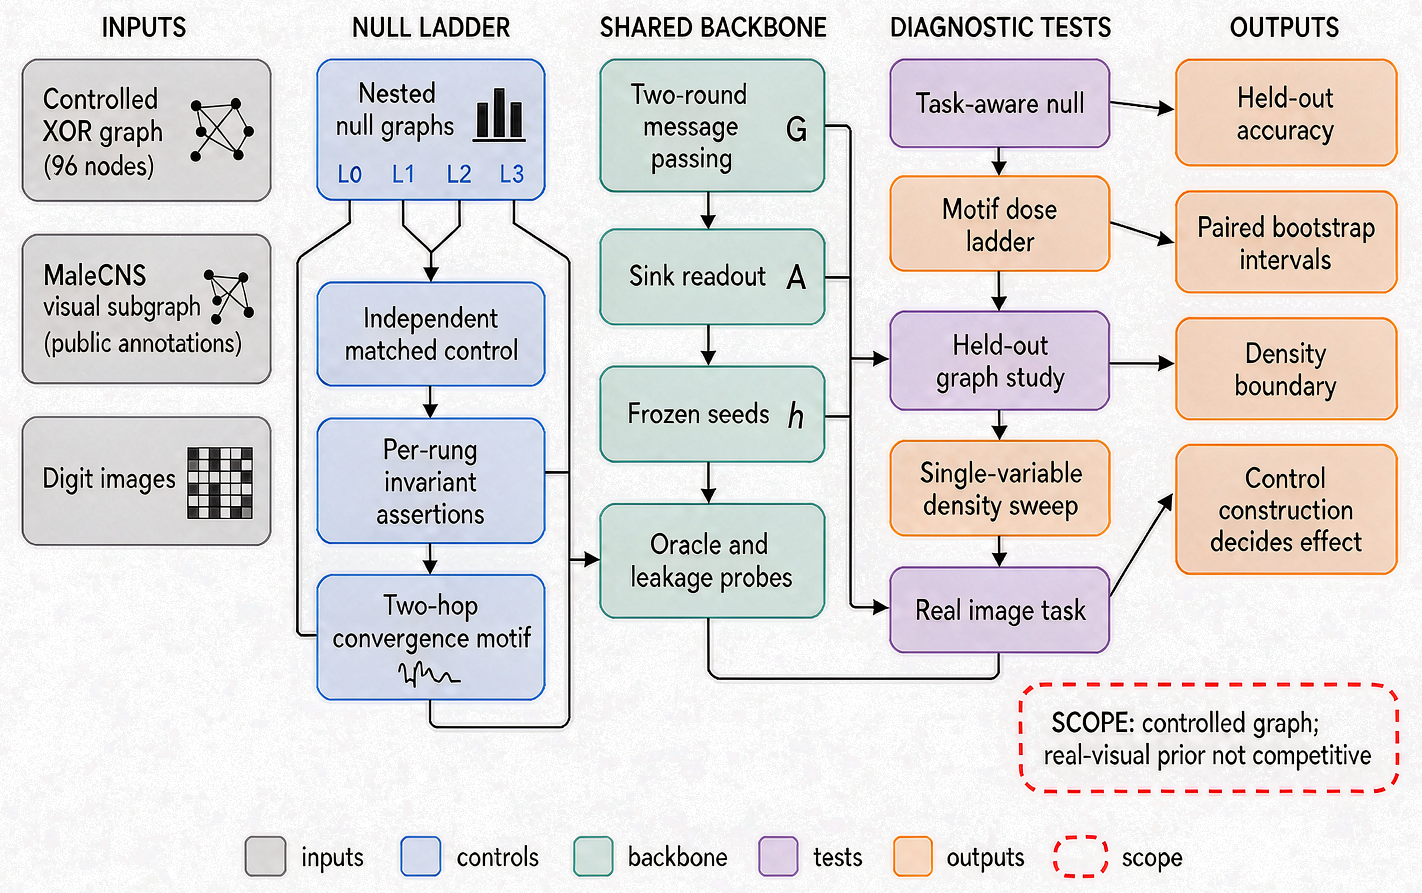
\includegraphics[width=0.92\linewidth]{figures/fig1_framework.png}
  \caption{Overall framework. A controlled two-hop XOR graph, a public
    MaleCNS v1.0 visual subgraph and digit images are evaluated under a
    nested null ladder with per-rung invariant assertions and a shared
    two-round message-passing backbone; diagnostic tests (task-aware null,
    motif-dose ladder, held-out study, density sweep, density$\times$survival
    grid, real image task) yield held-out accuracy with paired bootstrap
    intervals. The dashed box marks the scope conditions.}
  \label{fig:framework}
\end{figure}

Figure~\ref{fig:framework} summarises the design: the null generator, rather
than the graph family, is the experimental variable, and every condition
shares the same backbone, initialisation and seeds.

\begin{figure}[t]
  \centering
  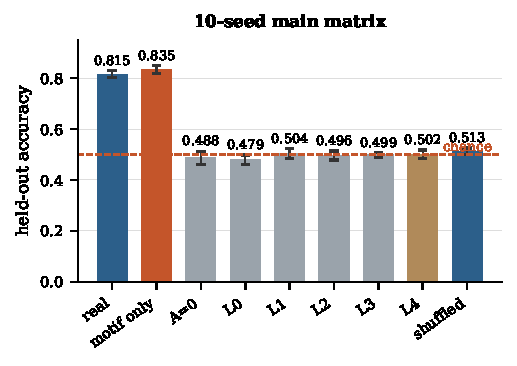
\includegraphics[width=0.9\linewidth]{figures/fig2_main_results.pdf}
  \caption{Ten-seed held-out accuracy. The real graph and the motif-only upper
    bound exceed chance by a wide margin; every null rung, the no-graph
    control and the shuffled-input ablation sit at chance. Error bars are
    seed standard deviations.}
  \label{fig:main}
\end{figure}

Table~\ref{tab:main} and Fig.~\ref{fig:main} summarise the campaign: the real
graph reaches $0.8152$ (seed variance $2.1\!\times\!10^{-4}$); the no-graph
control and all four rungs lie between $0.4795$ and $0.5039$, every
real-minus-condition difference is $0.30$--$0.34$ with 95\% intervals
excluding zero and BH $q=0.0002$. The motif-only graph slightly \emph{exceeds}
the full graph ($0.8348$, $\Delta=-0.0195$) -- the injected motif is the
information path and background edges add noise. Shuffling the node-to-input
mapping collapses accuracy to $0.5133$, ruling out a readout artefact.

The decisive observation is in the $\Delta$ column of Table~\ref{tab:main}: the
four nested rungs differ from one another by at most $0.0244$ in their
real-minus-rung delta, an order of magnitude less than the effect itself.
\textbf{The ladder has no localising power.} Matching degree, module blocks and
triad census removes the advantage to essentially the same extent as a plain
edge-count-matched random graph.

Table~\ref{tab:main} also reports, for each control, the surviving motif edges
$|P\cap A|$ and its global two-path match $\Delta_{\rm conv2}$ -- a \emph{post-hoc
re-analysis} of the same frozen null instances (no new training, seeds or label
access), outside the preregistered significance family. They expose the central
asymmetry: L1 matches the global statistic best ($0.13$) yet keeps only $1.13$
of 18 path edges and is at chance; L3 matches well ($0.50$), keeps $13.38$
edges, and is still at chance -- neither quantity alone orders accuracy. A
post-hoc oracle on the identical protocol reaches $0.7859$, ruling out an
unlearnable label; with a measured $6.06\%$ noise flip rate the ceiling is
$0.9395$, so an oracle near $1.0$ is unattainable here.

\subsection{Is survival count a sufficient statistic?}
\label{sec:survival}

A stronger hypothesis is that accuracy is a function of $|P\cap A|$ alone. A
\emph{post-hoc descriptive} check (not preregistered, no significance claim)
rejects it: a linear fit gives $R^2=0.10$; L2 ($13.50$ edges) and L3 ($13.38$)
retain most path edges yet stay at chance; decisively, the shuffled-input
ablation leaves the graph unchanged (all 18 edges) and still collapses to
$0.5133$. Path survival is \emph{necessary but not sufficient}: input--path
alignment is also required.

\subsection{Ladder statistics and invariant verification}
\label{sec:invariants}

Table~\ref{tab:invariants} reports maximum invariant violations: L1 preserves
degree exactly, L2 additionally preserves every module cell, and L3 reduces
the triad-census $L_1$ deviation to 20 from 1826 at L2 -- the generators do
what they claim. L4 violates every invariant (28 edges, 93 degree-mismatched
nodes, 39 module cells), confirming its reclassification as a control.

\begin{figure}[t]
  \centering
  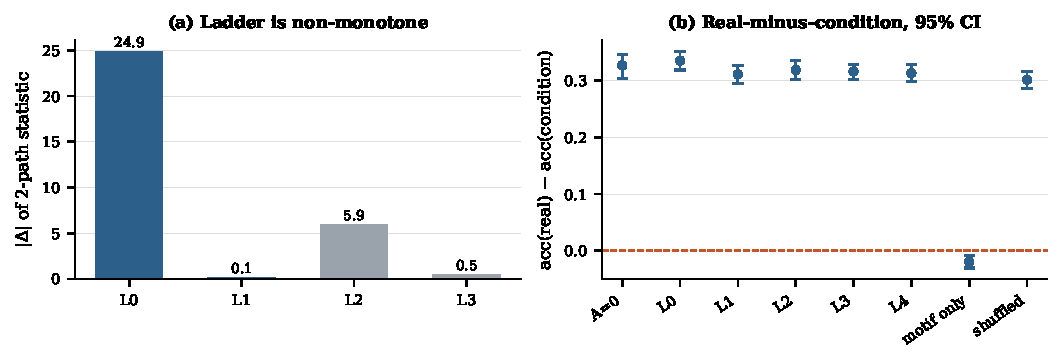
\includegraphics[width=0.94\linewidth]{figures/fig3_ladder_analysis.pdf}
  \caption{(a) Absolute mean difference of the two-path statistic from the
    real graph is non-monotone across L0--L3: degree preservation already
    matches the statistic; module and triad constraints do not tighten it
    further. (b) Paired accuracy differences with 95\% bootstrap intervals;
    all null conditions are statistically indistinguishable.}
  \label{fig:ladder}
\end{figure}

The two-path statistic confirms the picture (Fig.~\ref{fig:ladder}a):
absolute mean deviation $24.875$, $0.125$, $5.938$, $0.500$ for L0--L3 --
non-monotone with one inversion. Degree preservation alone reproduces the
global two-path count; higher-order constraints neither tighten it nor restore
the motif. The \emph{global} statistic is nearly matched by L1 while
\emph{accuracy} is at chance on L1: matching a graph statistic is not the
same as preserving the computational path.

\subsection{Robustness}
\label{sec:robust}

Table~\ref{tab:robust} reports $\mathrm{acc}(\text{real})-\mathrm{acc}(\text{L1})$
under two input-noise levels and two propagation depths; the effect persists
in all four cells ($0.1406$--$0.3652$) and degrades gracefully with noise,
consistent with a signal-to-noise rather than an artefactual origin. We
retain all four runs, including the weakest cell.

\subsection{Powered held-out prediction}
\label{sec:heldout}

An initial five-graph study produced only positive deltas, making sign
prediction unidentifiable; we therefore preregistered a powered follow-up
with \textbf{twenty} independently generated held-out graphs (ten intact,
ten with 75\% of motif edges removed). Deltas now span $-0.046$ to $0.372$
(12 positive, 8 non-positive). Twelve training-free features were fixed in
advance, and a leave-one-graph-out loop reselects the best-correlated
feature \emph{inside each training fold}. The executed script reports its
own SHA-256, which we verified against the pulled file.

Eight of twelve features remain significant after correction (Table~\ref{tab:heldout}):
two-path count, differential reachability, edge and module density, surviving
motif-edge count and fraction, and both source reachabilities. LOGO magnitude
prediction reaches MAE $0.1046$ against a constant baseline of $0.1635$ (36\%
better over twenty folds). \textbf{Sign agreement, however, is $0.60$ --
exactly the majority-class baseline.} This is consistent with the
dose--response threshold of \S\ref{sec:taskaware}: near the zero crossing,
which motif edges survive determines the sign, whereas global path statistics
vary smoothly with magnitude. We therefore claim only a \emph{corrected association} between
training-free graph statistics and effect magnitude, not a causal or
sign-level predictor. Because half the held-out graphs were deliberately
motif-degraded, several significant features (surviving motif-edge count and
fraction, reachability terms) partly encode the manipulation itself; they
validate the manipulation rather than discover an independent graph law.

\subsection{Task-aware null and motif dose--response}
\label{sec:taskaware}

Section~\ref{sec:theory} predicts that a control is sufficient only if it
preserves the structures the hypothesis does not ablate; we test this
constructively in a companion 10-seed run on the same graph and protocol. A
\emph{task-aware null} protects all 18 motif edges and randomises only the
background under the same degree and module-pair constraints; a \emph{strong
null} also removes all motif edges; a dose ladder deletes $0,4,9,14,18$ of the
18 motif edges. All conditions share the frozen seeds.

\begin{figure}[t]
  \centering
  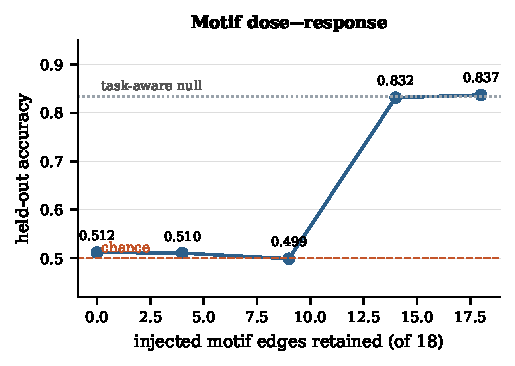
\includegraphics[width=0.9\linewidth]{figures/fig4_dose_response.pdf}
  \caption{Motif dose--response. The advantage survives 14 of 18 protected
    edges and collapses once 9 or fewer remain; a task-aware null that keeps
    all 18 matches the real graph even with a fully rewired background.}
  \label{fig:dose}
\end{figure}

Table~\ref{tab:taskaware} and Fig.~\ref{fig:dose} give the result. The
task-aware null reaches $0.8346$, statistically indistinguishable from the
real graph ($0.8371$; $\Delta=0.0025$, CI $[-0.0025,0.0084]$, $q=0.40$),
despite a fully rewired background. The strong null falls to $0.4920$ and
motif removal to $0.5117$ (both $q=0.00032$). The dose ladder is sharply
thresholded: $0.8371$, $0.8316$, $0.4988$, $0.5104$, $0.5117$ for
$18,14,9,4,0$ surviving edges. A background-only null that leaves 14 motif
edges intact ($0.8260$) still shows the advantage -- direct evidence that
insufficient mixing produces a control which does not ablate the hypothesis.

This closes the mechanism loop: the advantage is carried by a small,
identifiable subgraph, and \emph{how many} task-relevant edges a control
preserves -- not which rung it belongs to -- determines the measured effect.
Because this companion run is independent -- a freshly generated graph, a
separate execution, a pulled uncorrupted script -- it also reproduces the
main campaign's qualitative pattern (real $\approx\!0.84$ \emph{vs}.\
no-graph $\approx\!0.51$, paired CIs excluding zero, $q\!\approx\!0.0003$),
cross-validating \S\ref{sec:main} without erasing the execution defect
disclosed in \S\ref{sec:discussion}.

\subsection{External validation on a real MaleCNS visual subgraph}
\label{sec:realconnectome}

To test whether the controlled findings transfer to biological wiring, we
streamed the public 1.05\,GB MaleCNS v1.0 connectome weight table
(CC-BY~4.0~\cite{malecns2026}) with Arrow record batches and column
projection, selected 9{,}766 visually annotated body IDs from the 14.5\,MB
annotation file, and formed a 768-node induced subgraph over the
highest-degree visual neurons ($48{,}713$ edges after removing the ten
shortcut edges; $48{,}723$ before that removal in the companion run). The full matrix was never densified. A
genuine two-hop convergence motif -- two in-neighbours feeding a relay that
reaches eight downstream sinks -- was located in this real graph; no edges
were injected. We ran real / $A\!=\!0$ / degree-preserving / task-aware /
motif-removed conditions over six frozen seeds on the same GPU.

All five conditions remain at chance (Table~\ref{tab:real}) and every paired
interval contains zero. \textbf{The structure-sensitivity precondition of
\S\ref{sec:task} fails on this dense subgraph}: with mean in-degree
$\approx\!63$, neighbour-averaged propagation plausibly dilutes the two source
signals below the readout's resolution -- a hypothesis, since this run had no
oracle control; \S\ref{sec:density} supplies it. This is a boundary condition,
not a contradiction of the controlled result -- a diagnostic task must be
solvable on the real graph before any null comparison is interpretable. We
report the negative run in full and scope the controlled-graph conclusion to
low-in-degree, path-identifiable subgraphs.

A preregistered follow-up asked whether this failure came from graph density:
we sparsified the \emph{same real subgraph} by keeping the four
highest-weight in-edges per node ($48{,}723 \to 3{,}072$ edges, mean in-degree
$63.4 \to 4.0$; ten shortcut edges then removed). \textbf{Five settings
changed together} (top-4 sparsification, readout mean$\to$sum, width
$64\!\to\!128$, learning rate $0.006\!\to\!0.008$, epochs $120\!\to\!300$);
seeds, graph and motif were unchanged, so this follow-up \emph{cannot} isolate
density -- only establish that a solvable regime exists on real wiring. The
structure-sensitivity precondition is now satisfied (Table~\ref{tab:real},
``Sparse''): the real graph reaches $0.6423$, above $A\!=\!0$ ($0.5283$;
$\Delta=0.1139$, CI $[0.0485,0.1680]$) and above motif removal ($0.5160$;
$\Delta=0.1263$, CI $[0.0736,0.1608]$).

Yet the ladder behaves differently from the controlled graph. The
degree-preserving null \emph{retains} most of the advantage ($0.6162$;
$\Delta=0.0260$, CI $[-0.0348,0.0921]$, containing zero), while the
task-aware null gives $0.5850$ ($\Delta=0.0573$, CI
$[0.0059,0.1029]$). The preregistered motif-survival-threshold hypothesis is
therefore \textbf{not} confirmed on the real subgraph
, and we make no replication claim.
Together the two real-graph runs establish a sharper boundary: whether a null
removes the effect depends on the density and higher-order organisation of the
\emph{target} graph, not on the rung label alone. On the dense projection the
diagnostic task is not solvable at all; on its sparsified counterpart the
degree sequence already carries the task-relevant path. This is direct
empirical support for our central recommendation -- the structure-sensitivity
gate and control survival counts must be measured on the target graph, since
neither transfers from a controlled surrogate.

\subsection{Isolating density on real wiring}
\label{sec:density}

The five-setting follow-up above cannot attribute the change. We therefore ran
a \emph{single-variable} sweep on a freshly streamed real MaleCNS visual
subgraph (768 nodes, 44{,}815 edges, mean in-degree 58.35; 29{,}442 visually
annotated body IDs), holding the readout (mean), epochs (120), hidden width
(64), learning rate (0.006), six seeds and the two-hop motif fixed while
varying \emph{only} the number $k$ of retained in-edges per node. An oracle MLP
given both source features directly reaches $1.0000$ on all six seeds: the XOR
label is fully learnable on this graph, so the dense failure is a propagation
problem, not a label problem.

Table~\ref{tab:density} shows a sharp density threshold: the real graph stays
at chance for in-degree 58.4 / 49.0 / 15.9, rises to $0.6227$ at $8.0$, and
reaches $0.9863$ / $0.9987$ at $4.0$ / $2.0$, while $A\!=\!0$ and the
degree-preserving null stay near $0.50$ throughout; the task-aware null
recovers in parallel ($0.9027$ / $0.9971$ at $k\!=\!4/2$) -- the only echo on
real wiring of the controlled task-aware result. \textbf{Density alone
determines whether the gate passes}; it does \emph{not} establish motif
survival as the causal variable (at $k\!=\!4,2$ the protected edge
$23\!\to\!63$ is absent yet accuracy is near ceiling). We claim a density
boundary, not a transferred motif-survival threshold. Visual-ID matching
differs across runs, so absolute edge counts are not comparable between
\S\ref{sec:realconnectome} and this section; within the sweep all $k$ share
one graph and one motif.

\subsection{The two-factor gate: a pre-registered density$\times$survival grid}
\label{sec:grid}

The controlled campaign and the real-wiring sweep each isolate one factor:
path survival on a sparse controlled graph, wiring density on real biology.
If the factors gate jointly, raising the background density should close the
gate even when the path is fully protected, and destroying the path should
matter only while the background stays sparse. We preregistered exactly this
grid (config and analysis frozen before training) on the same 96-node graph
and protocol as \S\ref{sec:main}--\ref{sec:taskaware}: the background is
resampled at four density scales ($s\in\{1,8,32,64\}$; mean in-degree $1.5$
to $34.8$), the 18 motif edges are thinned to $k\in\{18,9,0\}$ survivors,
and six paired seeds provide seed-paired effects against the no-graph control
with bootstrap intervals.

\begin{figure}[t]
  \centering
  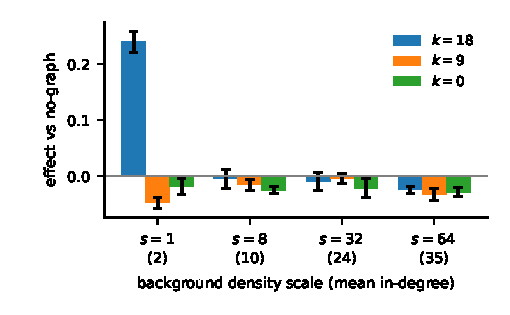
\includegraphics[width=0.9\linewidth]{figures/fig6_density_survival_grid.pdf}
  \caption{Pre-registered density$\times$survival grid on the controlled
    graph family. Effect $=$ held-out accuracy minus the paired no-graph
    control, mean over six frozen seeds; error bars are seed standard
    deviations. The advantage requires \emph{both} a protected path and a
    sparse background: at the highest density even $k=18$ sits at chance,
    and at the base density $k=9$ already collapses.}
  \label{fig:grid}
\end{figure}

Table~\ref{tab:grid} and Fig.~\ref{fig:grid} give the result. All three
preregistered predictions hold: the base graph replicates the main effect;
the effect falls monotonically with background density at full survival; and
the interaction is decisive -- $k{=}18$ at the highest density sits at or
below the no-graph control, while $k{=}9$ already collapses at base density.
\textbf{Neither factor rescues the other}: a protected path is diluted below
readout resolution by a dense background, and a sparse background cannot
transmit a label through a destroyed path. This converts the cross-system
disagreement of \S\ref{sec:intro} into a prediction: comparisons on sparse,
path-identifiable circuits should show an advantage that null ladders cannot
localise, while projections of the dense connectome should show a null --
exactly the published pattern.

\subsection{A real visual task: a negative boundary}
\label{sec:visualtask}

To test whether the connectome prior is a competitive visual bias, we ran a
real image-classification task (scikit-learn digits, real $8\times8$
handwritten digits, 10 classes, fixed 1078/359/360 split) through a 768-node
MaleCNS visual subgraph, comparing the real graph, a degree-preserving null,
$A\!=\!0$, a task-aware null and a non-graph MLP over six seeds. An MNIST
add-on used the same protocol.

The real graph significantly beats no graph ($+0.0995$, CI
$[0.0556,0.1648]$), but the degree-preserving null matches it exactly
($-0.0005$, CI $[-0.0412,0.0440]$), and a plain MLP dominates every graph
model ($0.9722$ vs $0.7185$; MNIST: $0.8879$ vs $0.7649$).
\textbf{We report this as a negative result}: on these tasks the wiring prior
is not a competitive inductive bias, and the gain over no graph is already
explained by the degree-preserving control. A consistency caveat: on MNIST
the real graph \emph{does} beat the degree-preserving null by a small but
significant margin ($+0.0148$, CI $[0.0100,0.0192]$), opposite in sign to
the digits result. We report both: null behaviour is dataset-dependent, which
further supports measuring the gate and survival counts on the target task.

\section{Discussion}
\label{sec:discussion}

\paragraph{Relation to the strongest published control ladder.}
The closest prior work~\cite{toposens2026} introduces a staged \emph{control
ladder}: an apparent early-training advantage that disappears under shared
random initialisation and a degree-preserving null. Our protocol \emph{begins}
at that strict endpoint and supplies the axes their limitations name as future
work -- higher-order rungs, full convergence, corrected multi-seed statistics
-- plus an explicit record of which task-relevant edges each control preserves
(we did not rerun their flyvis stack). Under our protocol the degree-preserving
null removes the advantage, yet a task-aware null restores it
(\S\ref{sec:taskaware}): degree preservation is not the endpoint of control
strength -- preservation of the computational path is.

\begin{figure}[t]\centering\refstepcounter{auditbox}\label{alg:audit}
\fbox{\parbox{0.955\linewidth}{\footnotesize
\textbf{Algorithm \theauditbox: survival-count audit.}\par\vspace{2pt}
\textbf{(1) Gate:} verify structure sensitivity with an $A{=}0$ control, a
leakage probe and an oracle on the label-defining inputs; stop if the label
is unlearnable. \textbf{(2) Localise:} ablate to find the minimal edge set $P$
whose removal destroys the only information path. \textbf{(3) Count:} report
$|P\cap C|$ for every control $C$ beside the delta -- Eq.~\eqref{eq:survival}
predicts unprotected edges vanish under mixing, so this count, not the rung
label, is informative. \textbf{(4) Decide:} $C$ is \emph{sufficient} only if it
preserves everything the hypothesis does not ablate. Do not skip (1):
survival is necessary but not sufficient (\S\ref{sec:survival}).}}
\end{figure}

\paragraph{A two-factor reading of the cross-system disagreement.}
The grid supplies a coordinate system for the literature of
\S\ref{sec:intro}, not a rebuttal of any single study. Reservoir-style nulls
from projections of tens of thousands of synapses onto a small
input/output set~\cite{larvanull2026} sit in the dense-background regime where
our gate predicts a null regardless of path survival; advantages on sparse,
cell-type-resolved visual circuits~\cite{structurealone2026} sit in the sparse
regime where a protected path survives ordinary nulls. We did not recompute
any prior study's graph, and the mechanism governs neighbour-averaged message
passing with pooled readout: models that learn per-edge gains, or read out
from designated neurons rather than a pooled average, can escape the dilution
gate. The larval study's own record is instructive either way -- a suggestive
$n{=}5$ effect ($p{=}0.078$) that evaporated at $n{=}15$ is the winner's-curse
dynamic that frozen multi-seed protocols exist to prevent~\cite{larvanull2026}.

\paragraph{How to repair your null.}\label{sec:repair}
Fix every edge of $P$, then apply the degree- and module-preserving swap chain
to the \emph{remaining} edges only. This is $L^*$ (Table~\ref{tab:taxonomy}):
invariants stay comparable to L1--L3 while one factor varies -- whether $P$
survives. The companion run (\S\ref{sec:taskaware}) shows this single change
moves accuracy from chance to $0.8346$, indistinguishable from the real
graph. The recipe applies to mechanistic and learned-gain models alike.
Algorithm~\ref{alg:audit} operationalises it by reusing the controls a study
already computes and adding only an edge-intersection count;
Table~\ref{tab:literature} applies the same reading aid to the motivating
works; all entries are \emph{we estimate / proxy} statements, not claims that
a prior conclusion is wrong.

\paragraph{Limitations.}
\emph{Scope}: an evaluation-methodology study with no image benchmark, no
natural visual task and no claim of improved visual accuracy; all results are
stated as conditions on control construction, never as a visual-accuracy gain.
\emph{Data}: the main results use a 96-node controlled graph; the density
$\times$survival grid (\S\ref{sec:grid}) uses the same single realization with
six seeds -- it demonstrates the interaction on one controlled family, not its
quantitative form across graphs; the real 1.05\,GB MaleCNS runs are boundary
conditions, not replications (\S\ref{sec:realconnectome}--\ref{sec:visualtask}). \emph{Baselines}: flyvis and the published shared-initialisation pipeline
were not rerun; L1 implements the degree-preserving idea only; signed/typed
edges were not modelled.
\emph{Statistics}: sign prediction equals the majority baseline, so only
magnitude association is supported. \emph{Protocol}: the three-seed pre-check remains
\emph{failed} with a documented probe defect; one early aggregation block
crashed after flushing all data (LOGO values were recomputed from the recorded
rows) and its executed script does not match the recorded checksum, whereas
all later runs have verified script hashes. \emph{Comparability}: real-subgraph
runs use different visual-ID matchings (9{,}766 / 29{,}442 / 29{,}564 IDs), so
absolute edge counts are not poolable. All runs, including negative ones, are
retained; the real-image study serves as a scope boundary for the claim.

\paragraph{Reproducibility.}
Frozen seeds, hyperparameters, executed scripts, metrics, per-seed logs and
invariant counts are preserved; all tables and figures derive directly from
the recorded measurements; the real-subgraph runs have verified
executed-script checksums (dense \texttt{090d9535\ldots}, sparse
\texttt{026bf88e\ldots}, sweep \texttt{360a3808\ldots}, visual \texttt{28f5744d\ldots}). The
failed pre-check and transfer-repair records are retained.

\paragraph{Ethics and broader impact.}
Purely computational: no human subjects, animal work or deployed system; the
only biological input is a public CC-BY~4.0 annotation file (credited). The
misuse risk is the one documented here -- an inadequately specified null
yields a confident but wrong structural attribution -- hence the survival-count
recommendation.

\section{Conclusion}
\label{sec:conclusion}

We asked when connectome wiring helps visual computation, and answered with a
mechanism rather than a verdict. On controlled sparse circuits, topology
confers a large advantage that no ladder of global-statistic nulls can
localise, because the operative variable is whether the control preserves the
task-relevant path. On real MaleCNS wiring, in-degree alone gates whether the
task is solvable, and the preregistered density$\times$survival grid confirms
that the two factors interact: a dense background erases even a protected
path, and a sparse one cannot rescue a destroyed one. The mechanism reframes
the conflicting literature as coordinates of one plane and delivers a
practical standard: measure the gate and count surviving path edges before
believing any structural attribution.

\clearpage

\section*{LLM Usage Statement}
Large language models were used during the preparation of this manuscript as
a writing and editing assistant, including drafting support, language
polishing, and \LaTeX{} formatting of the text. The research questions,
experimental design, implementation, execution, numerical results, and
statistical analysis are the authors' own work; the authors verified every
reported number against the recorded run data and reviewed all AI-assisted
passages for accuracy. The authors take full responsibility for the content
of this paper, and no AI system is listed as an author.

{
\small
\bibliographystyle{ieeenat_fullname}
\bibliography{main}
}

\end{document}
